\subsection{Fysiske konsekvenser ved aktivitet}
Fysisk aktivitet er defineret som enhver bevægelse, hvor skeletmuskler skal kontrahere og derved forbrænde energi. Der er forskellige former for fysisk aktivitet, som har forskellige intensitetsniveauer. \citep{Academic2016a} Ifølge Sundhedsstyrelsen skal et barn i alderen 5-17 år være fysisk aktiv i mindst 60 minutter om dagen med moderat til høj intensitet. Derudover anbefales det, at børn i denne alder skal indgå i en aktivitet i 30 minutter med høj intensitet tre gange om ugen. \citep{Sundhedsstyrelsen2016} Hvis Sundhedsstyrelsens anvisninger følges, kan der opnås åbenlyse fordele. Fysisk aktiviteten kan mindske risikoen for flere alvorlige kroniske sygdomme som diabetes og hjertesygdomme. Derudover er fysisk aktivitet forebyggende for en række følgesygdomme, som kan opstå af inaktivitet. Det udvikler og styrker barns led, knogler og muskler. Dette er blandt andet et resultat af, at under fysisk aktivitet frigiver kroppen hormoner, som sætter gang i forskellige processer. Eksempelvis dannes der mere synovialvæske, hvorved bevægelse af led faciliteres. Knogler vedligeholdes af fysisk aktivitet, hvorved der undgås, at knoglens densitet mindskes som beskrevet i \secref{subsec:inover}. Muskler udvikles og vedligeholdes ligeledes af fysisk aktivitet, men afhænger af aktivitetens type. Overvægt kan både forbygges og behjælpes af fysisk aktivitet, da det opstår ved, at der indtages mere energi end der bliver brugt. Aktivitet medfører forbrænding af denne indtagede energi, hvorved ligevægtsindtaget muligvis ikke overskrides. \citep{Academic2016a,Smith1991,Academic2016b,Cotman2007,CenterforDiseaseControlandPrevention2015}

Kroppen har mange reaktioner på fysisk aktivitet, hvilket blandt andet afhænger af aktivitetens krav til kroppen\fxnote{Skal muskelgrupper fremskynde en position som ved svømning og derved være udholdende eller skal muskelgrupper løfte en vægt som ved vægtløftning og derfor være eksplosiv men knap så udholdende?} og intensiteten heraf. Ved anstrengende fysisk aktivitet overtager sympatikus størstedelen af det autonome nervesystem og sætter for eksempel fordøjelsen på pause, da fordøjelse ikke længere er førsteprioritet og al kroppens energi kan bruges til aktivering af de pågældende skeletmuskler. Hjertet slår hurtigere, hvilket gør at pulsen stiger, hvorved ilt og næringsstoffer hurtigere sendes rundt i kroppen \citep{Hjerteforeningen}. Blodkar vil spile ud, så blodet i større grad kan komme til hudoverfladen og afgive den varme, som blodet fører fra de bevægende muskler. Der sker altså en stigning i pulsen og blodtrykket, og denne stigning afhænger af den pågældende aktivitets påvirkning på kroppen. \citep{Martini2012,Stanfield2013,Berchtold2010}

\subsection{Fysiske konsekvenser ved aktivitet} \label{subsec:fysio_aktivitet}
Fysisk aktivitet er defineret som enhver bevægelse, hvor skeletmuskler skal kontrahere og derved forbrænde energi. Der er forskellige former for fysisk aktivitet, som har forskellige intensitetsniveauer. \citep{Academic2016a} Ifølge Sundhedsstyrelsen skal et barn i alderen 5-17 år være fysisk aktiv i mindst 60 minutter om dagen med moderat til høj intensitet. Derudover anbefales det, at børn i denne alder skal indgå i en aktivitet i 30 minutter med høj intensitet tre gange om ugen. \citep{Sundhedsstyrelsen2016} Hvis man følger sundhedsstyrrelsens anvisninger, vil man som resultat af aktiviteten, opnå åbenlyse foredele. Aktiviteten kan mindske risikoen for flere alvorlige kroniske sygdomme som diabetes og hjertesygdomme. Fysisk aktivitet er ikke kun forebyggende for en række følgesygdomme af inaktivitet. Det både udvikler og styrker det aktiverede barns led, knogler og muskler. Dette er blandt andet et resultat af, at under fysisk aktivitet frigiver kroppen hormoner, som sætter gang i forskellige processer. Eksempelvis dannes der mere synovialvæske, hvorved bevægelse af led faciliteres. Knogler vedligeholdes af aktiviteten, og man udgår knoglens densitet mindskes. Muskler udvikles og vedligeholdes ligeledes af aktiviteten, dog afhængigt af aktivitetens type. Fysisk aktivitet er en af faktorerne til både at forebygge eller behjælpe overvægt. Overvægt er som nævnt, et resultat af at der indtages mere energi end der bliver brugt. Aktivitet medfører at noget af denne energi forbrændes, og at ligevægtsindtaget muligvis ikke overskrides. \citep{Academic2016a,Smith1991,Academic2016b,Cotman2007,CenterforDiseaseControlandPrevention2015}

Der findes en klar sammenhæng imellem puls og kroppens reaktion på motionen. Ifølge flere studier hænger procenten af den maksimale puls sammen med, antallet af forbrændte kalorier, om den aerobe udholdenhed trænes, forbedrer den anaerobe tolerance eller forbedrer den cardiovaskulære ydeevne\fxnote{hvilket gør, at man kan sprinte længere / er hurtigere, fordi der kommer mere ilt rundt i kroppen}. Jo højere procent intensitet, desto højere puls og hårdere fysisk træning. Denne sammenhæng inddeles i zoner som ses på \figref{fig:PA_Procentpuls}. \citep{Leyland2007,Heartratejournal2015}
\begin{figure}[H]
	\centering
	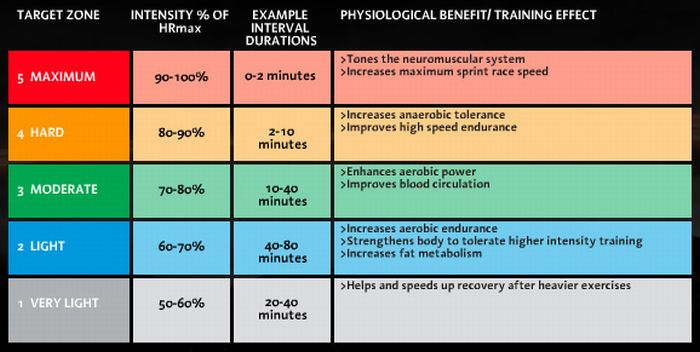
\includegraphics[scale=0.75]{figures/aProblemanalyse/heart-rate-zones.jpg}
	\caption{På figuren ses fem zoner for kroppens reaktion i forhold til pulsraten. Der ses, at de fem zoner har hver sin påvirkning på kroppen. Det er dog også anbefalet, at varigheden i hver zone bliver lavere desto hårdere aktiviteten er. \citep{Heartratejournal2015}}
	\label{fig:PA_Procentpuls}
\end{figure}

Det er dog omdiskuteret, hvorvidt zone 1 og 2 er de fortrukne, hvis ønsket er at tabe sig. Der forbrændes flere kalorier ved højintens aktivitet, altså i zone 4-5. I de lavintense zoner forbrændes kalorier fra fedtceller istedet for glykogen fra muskler, hvorfor kroppen efterfølgende vil lagre kalorier i fedtcellerne, som lider underskud. Hvis man derimod dyrker højintens arbejde, som svarer til zone 4 eller 5, vil glykogenen i musklerne forbrænde, og kalorier sendes derfor til musklerne, så de kan repareres og fortsætte arbejdet. De højintense zoner kan oftest ikke opretholdes over lang tid. \fxnote{Moderat intensitet svarer til 40-59\% af den maksimale iltoptagelse, eller 40-59\% af pulsreserven (maxpuls – hvilepuls), eller 64-74\% af maxpuls eller 12-13 RPE (rate of percieved excertion, Borgskala) og er yderligere defineret som fysisk aktivitet hvor man bliver lettere forpustet men hvor samtale er mulig. \citep{Kiens2007}} \citep{Martini2012,Leyland2007,Heartratejournal2015}. \newline
Pulsen er altså en faktor, som er medbestemmende for aktivitetens fokus. Dette medfører at pulsen er bestemmende for intensiteten, varigheden og udbyttet.

\subsubsection{Gængse aktivitetsformer blandt børn}

%  OBS: Generelt - vi skal have flyttet den defination vi snakkede om.
%  OBS: Vi skal måske lige snakke om relevansen for dette afsnit
%		Det eneste formål vi ønsker med dette afsnit er 'At sikre hvorfor vi ønsker 
%       de krav som vi gør. --> Burde det så ikke bare være et kort afsnit inde i 
%       opstillingen af succeskrav
%
%	Hvis afsnittet skal være her, er dette en mulig opstilling med indhold.
%	
%	Afsnittets opbygning: 
%	- Nævn betegnelsen inaktivitet og anbefalet aktivitet --> Skal lede op til: Hvad skal man egentlig lave så?
%	- Opremsning af aktiviteter som hører under moderart til høj intensitet -> aktivitet som ville være fordelagtige at udeføre for at opnå anbefalingerne.
%		- Tabel fra sundhedsstyrrelsen nævner mange til som børn bør lave som ville 
%		  aktivere dem nok til at få nok ud af motionen (Foldbold, cykling, leg i skolegård)
%		- Disse aktiviteter skal blandt andet ligge til grundlag for senere valg af krav
%		- Disse aktiviteter skal definere 'gængs aktivitet blandt skolebørn' (Uden at gøre det for groft, = Gang, løb og cykling bør dække nævnte aktiviteter)
%		- https://sundhedsstyrelsen.dk/da/sundhed-og-livsstil/fysisk-aktivitet/anbefalinger/~/media/31FF5ED226F643D0A6948B52948E5DB3.ashx
% 	- Argument for cykling er/bør være en gængs aktivitet
% 		- Giver øget koncentrationsevne+indlæringsevne 
%		- Børn der cykler er sundere
%		- https://www.cyklistforbundet.dk/Om-os/Vi-mener/Cyklistforbundet-mener/Boerns-cykling-til-skole-og-i-fritiden
%	- Opsummering af hvorfor dette er/bør være gængs aktivitet for et barns hverdag
%	  og hvordan det påvirker børn rent fysiologisk.
		

%
%
	% Sundhedsstyrrelsens anbefalinger, sygdomme det hjælper på, fortsat af notater.
% Opbygning af afsnit %%%%%%%%%%%%%%%%%%%%%%%%%%%%%%%%%%%%%%%%%%%%%%
%-- Inaktivt og/eller overvægtig
% Kort introduktion, beskrivelse af hh. inaktivitet og overvægt.
% Følgesygdomme fra begge
% Sammenligning (Hvad er farligst, hvad er forskellen)
%-- Aktivt
% Kort introduktion, hvad betyder det at være aktiv(definition)
% Hvilken betydning har puls for forbrænding?
% Helbred 
%-- Kongnitiv funkktion (indlæring/Koncentration)
% Inaktivitet, overvægt og aktivitets påvirkning af kongitiv funktion (I hvor lang tid kan aktivitet hjælpe på indlæring?)
% Hvornår skal man være aktiv i forhold til undervisning?